\documentclass[14pt]{extreport}
\usepackage{ifluatex}
\ifluatex
    \usepackage{fontspec}
    \setmainfont{Literaturnaya}
    \setsansfont{Segoe UI}
    \setmonofont{MesloLGS Nerd Font Mono}
\else
    \usepackage[utf8]{inputenc}
    \usepackage[T1,T2A]{fontenc}
    \usepackage{literat}
\fi
\usepackage[russian]{babel}
\usepackage[os=win]{menukeys}
\renewmenumacro{\keys}{shadowedroundedkeys}
\renewmenumacro{\menu}{roundedmenus}
\renewmenumacro{\directory}{pathswithfolder}
\usepackage[title,titletoc]{appendix}
\usepackage{tocloft}
\renewcommand{\cftsecaftersnum}{.}
\renewcommand{\cftsubsecaftersnum}{.}
\usepackage{vmargin}
\setpapersize{A4}
\setmarginsrb{2.0cm}{1.0cm}{1.5cm}{1.5cm}{0pt}{0mm}{0pt}{15mm}
\usepackage{setspace}

\usepackage[ampersand]{easylist}
% \ListProperties(Numbers1=a,FinalMark1={)})
\setcounter{secnumdepth}{2}
\usepackage{indentfirst}
\graphicspath{ {./img/} {./PDF/} }
\usepackage[labelsep=period]{caption}
\usepackage{xcolor}
\usepackage{hyperref}
\definecolor{linkcolor}{HTML}{FF0000} % цвет ссылок
\definecolor{urlcolor}{HTML}{0000FF} % цвет гиперссылок
\hypersetup{pdfstartview=FitH,linkcolor=linkcolor,urlcolor=urlcolor,colorlinks=false}
\usepackage[normalem]{ulem} % для подчёркиваний uline
\ULdepth=0.2em
\sloppy

%Предопределенние приложений

\renewcommand{\thepart}{\arabic{part}}
\renewcommand{\thesection}{\arabic{section}}
\renewcommand{\thesubsection}{\thesection.\arabic{subsection}}

%Колонтитулы
\usepackage{fancyhdr}
\pagestyle{fancy}
\fancyfoot[C]{\thepage} %номер страницы слева сверху на четных и справа на нечетных
\renewcommand{\headrulewidth}{0.4pt}
\renewcommand{\footrulewidth}{0.4pt}
\renewcommand{\headsep}{30pt}
\renewcommand{\footskip}{25pt}
\fancyhead[L]{\textsf {Layout-GOST}}
\fancyhead[R]{\textsf {\href{https://www.google.com/search?q=\%23layoutgost}{\uline{\#layoutgost}}}}
\begin{document}
\begin{titlepage}

	\begin{figure}
		\vspace{-7ex}
		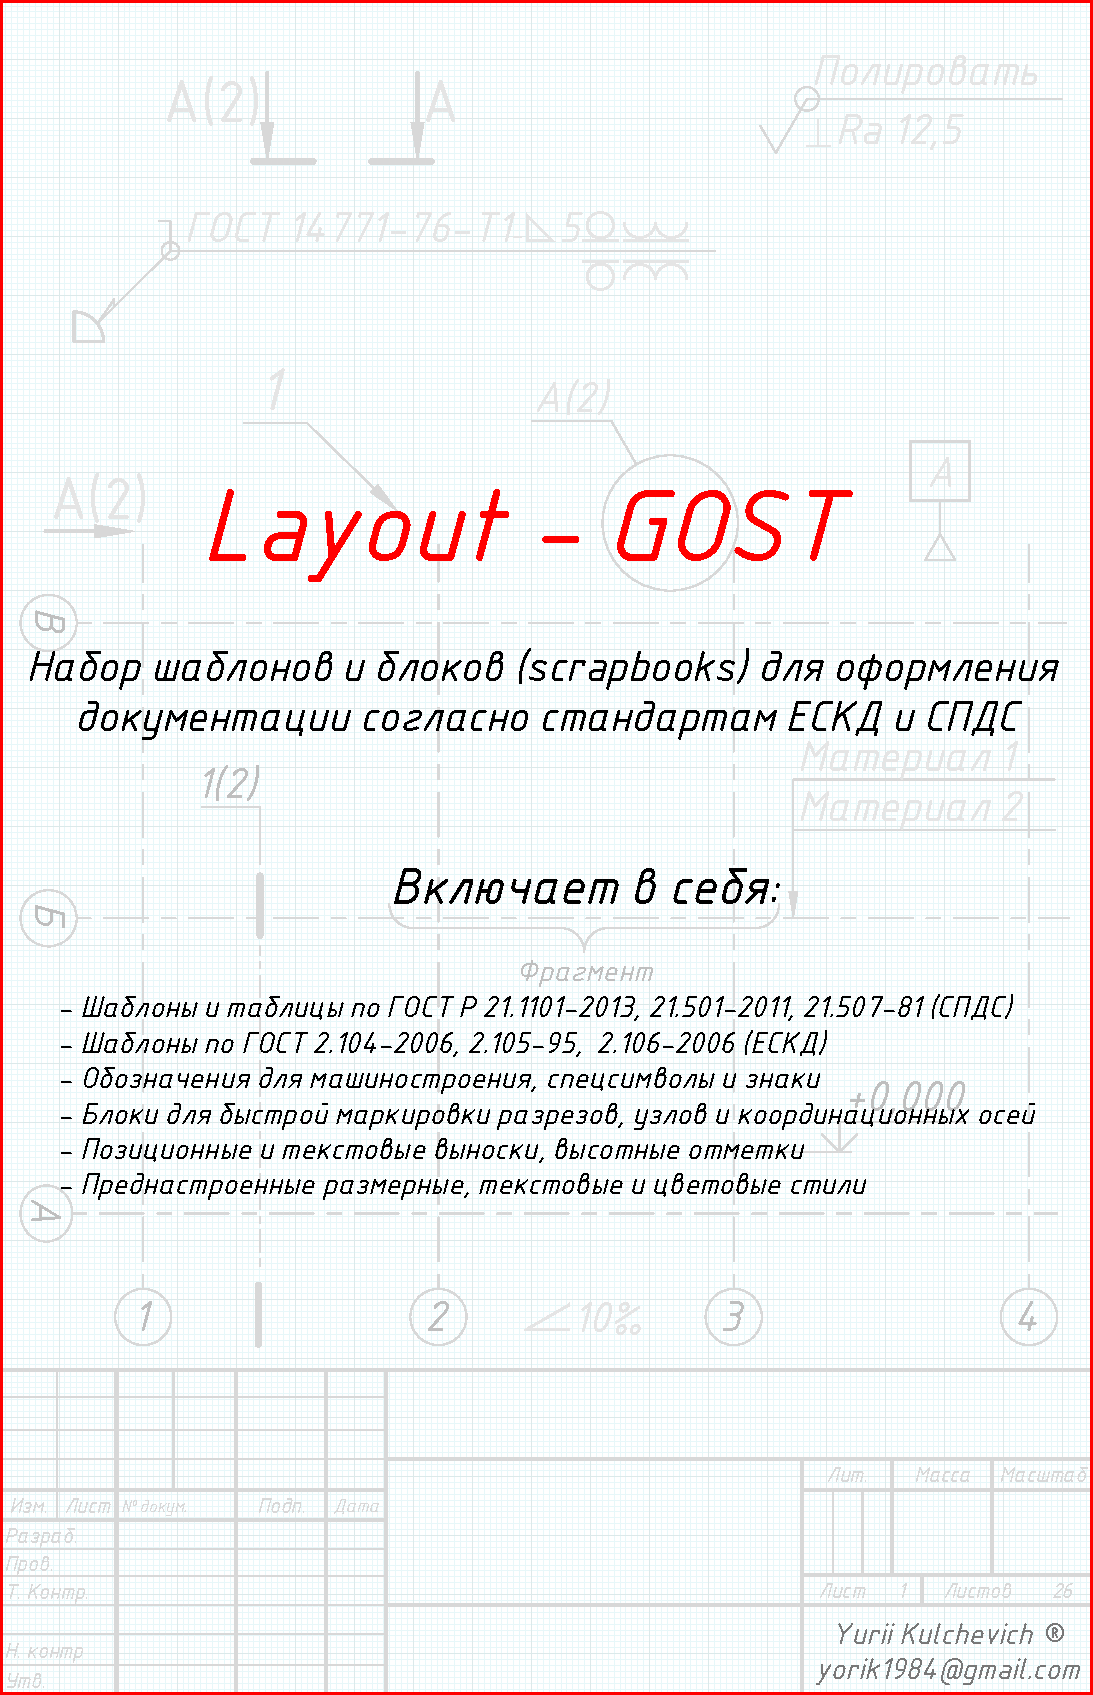
\includegraphics[width=185mm]{Layout-GOST_Title}
	\end{figure}

\end{titlepage}

\clearpage

\begin{doublespace}
    \tableofcontents
\end{doublespace}

\newpage

\section{Описание}
~\label{Opisanie}

Набор шаблонов и блоков (scrapbooks) Layout для оформления конструкторской документации согласно стандартам ЕСКД и СПДС включает:

\subsection{ЕСКД--шаблоны}

\begin{enumerate}
	\item Чертежи. Формат: А4, А3, А2. Ориентация листов альбомная (\textsf{L\_CHERTEZH}) и книжная (\textsf{P\_CHERTEZH}). Основная надпись по ГОСТ~2.104--2006 (Формы 1, 2 и 2а).
	\item Титульный лист А4 (\textsf{P\_TIT\_LIST}) по ГОСТ~2.105--95.
	\item Спецификация А4 (\textsf{P\_SPECIF}), Ведомость спецификаций А3 (\textsf{L\_VEDOMOST\_SPECIF}), Ведомость ссылочных документов А4 (\textsf{P\_VEDOMOST\_DOC}), Текстовый документ А4 (\textsf{P\_TEXT\_DOC}) по ГОСТ~2.106--96 (Формы 1, 3, 4, 9 соответственно). Основная надпись по ГОСТ~2.104--2006 (Формы 2 и 2а).
	\item Групповая спецификация А4 (\textsf{L\_SPECIF\_GROUP}), Групповая ведомость спецификаций А4  (\textsf{L\_VEDOMOST\_SPECIF\_GROUP}), Групповая ведомость ссылочных документов А4 (\textsf{L\_VEDOMOST\_DOC\_GROUP}) по ГОСТ~2.113--75 (Формы 1 и 1а, 3 и 3а соответственно).  Основная надпись по ГОСТ~2.104--2006 (Формы 2 и 2а).
	\item Шаблоны без основной надписи (\textsf{EMPTY}).
\end{enumerate}

\subsection{СПДС--шаблоны}

Оформлены согласно ГОСТ~21.1101--2013.
\begin{enumerate}
	\item Строительные чертежи основных комплектов. Формат А3, А2, А1 (\textsf{OSN\_DOC}). Ориентация альбомная (Приложение «Ж», формы 3 и 6).
	\item Строительные изделия. Формат А3, А2, А1 (\textsf{STR\_IZD}). Ориентация альбомная (Приложение «Ж», формы 4 и 6).
	\item Текстовых документов А4 (\textsf{P\_TEXT\_DOC}). Ориентация листов книжная (Приложение «Ж», формы 5 и 6).
	\item Обложка А4 (\textsf{OBLOZHKA}). Ориентация книжная (Приложение «Н», форма 12).
	\item Титульный лист А4 (\textsf{TIT\_LIST}).Ориентация книжная (Приложение «П», форма 13).
	\item Шаблоны без основной надписи (\textsf{EMPTY}).
\end{enumerate}

\subsection{Scrapbooks}
\begin{enumerate}
	\item \textbf{ЕСКД. Обозначения.} \textsf{GOST\_ESKD}.\\
	      Обозначение разрезов, направления взгляда, выносных элементов, выноски, обозначения шероховатости, осевые и центровые линии, неразъемные соединения, допуски формы, специальные символы.
	\item \textbf{ЕСКД. Основные надписи.} \textsf{GOST\_ESKD\_Osnovnye\_Nadpisi}.\\
	      Основные надписи по ГОСТ~2.104--2006 формы 1, 2, 2а и дополнительные графы к ним.
	\item \textbf{СПДС. Обозначения.} \textsf{GOST\_SDPS}.\\
	      Координационные оси, обозначение разрезов и узлов, выноски, маркеры, высотные отметки.
	\item \textbf{СПДС. Основные надписи.} \textsf{GOST\_SPDS\_Osnovnye\_Nadpisi}.\\
	      Основные надписи по ГОСТ~21.1101--2013 формы 3, 4, 5, 6 и дополнительные графы к ним.
	\item \textbf{СПДС. Таблицы.} \textsf{GOST\_SPDS\_Tablicy}:
	      \begin{easylist}
		      & Ведомость	рабочих чертежей основного комплекта (спецификаций), Ведомость ссылочных и прилагаемых	документов, Спецификация, Групповая спецификация, Состав проектной документации по ГОСТ~21.1101--2013 формы 1, 2, 7, 8, 14 соответственно;
		      & Ведомость отделки помещений, Экспликация помещений, Ведомость перемычек, Экспликация полов, Ведомость деталей, Спецификация на изделие, Групповая спецификация на изделие, Ведомость отделки фасада, Спецификация элементов перемычек, Спецификация элементов заполнения проемов по ГОСТ~21.501--2011 формы 1, 2, 3, 4, 6, 7, 8, 9 соответственно;
		      & Ведомость отделочных и лакокрасочных материалов по ГОСТ~21.507--81.
	      \end{easylist}
	\item \textbf{Палитра.} \textsf{Base\_Set}\\
	      Предварительно настроенные размерными стили, цвета, типы линий. Цвет всех элементов в \textsf{Scrapbooks} выбран произвольно и смысловой нагрузки не несет.
\end{enumerate}

\newpage

\section{Базовые настройки}
В шаблонах и блоках использованы следующие настройки шрифта и линий:
\begin{itemize}
	\item Единицы измерения, линейные --- миллиметры, точность 0,1~мм~(ЕСКД) и 1~мм~(СПДС)
	\item Единицы измерения, угловые --- градусы, точность $0,1^\circ$~(ЕСКД) и $1^\circ$~(СПДС)
	\item Основная линия --- 1,5 pts (0,55 мм)
	\item Тонкая линия, в т.ч. размерная и линия выноски --- 0,6 pts (0,2 мм)
	\item Засечки линейных и угловых размеров, длинна --- 3 pts (3,5 мм)
	\item Точка выноски, диаметр --- 2 pts (0,7 мм)
	\item Шрифт \textit{GOST Common} (прилагается к набору отдельно), начертание --- \textit{italic}
	\item Высота размерного текста и текста технических требований --- 14 pt (3,5 мм)
	\item Высота текста выноски --- 20 pt (5 мм)
	\item Высота текста основной надписи, в зависимости от типа --- 10pt (2,5 мм), 14pt (3,5 мм), 20pt (5 мм)
\end{itemize}

\section{Установка}
Скопировать каталоги \texttt{Templates} и \texttt{Scrapbooks} из установочного архива в каталог по данному пути для Windows 10 или аналогичный для других ОС:\\

\noindent
{\small \directory{C:/Users/<User>/AppData/Roaming/SketchUp/<SketchUp\_current>/LayOut}}

\section{Использование}
\subsection{Шаблоны}
При создании нового документа нужно выбрать шаблон. Пример выбора шаблона для стандартов ЕСКД и СПДС показан на Рис.~\ref{ESKD_NEW_FILE} и Рис.~\ref{SPDS_NEW_FILE} соответственно.

\begin{figure}[t]
	\centering
	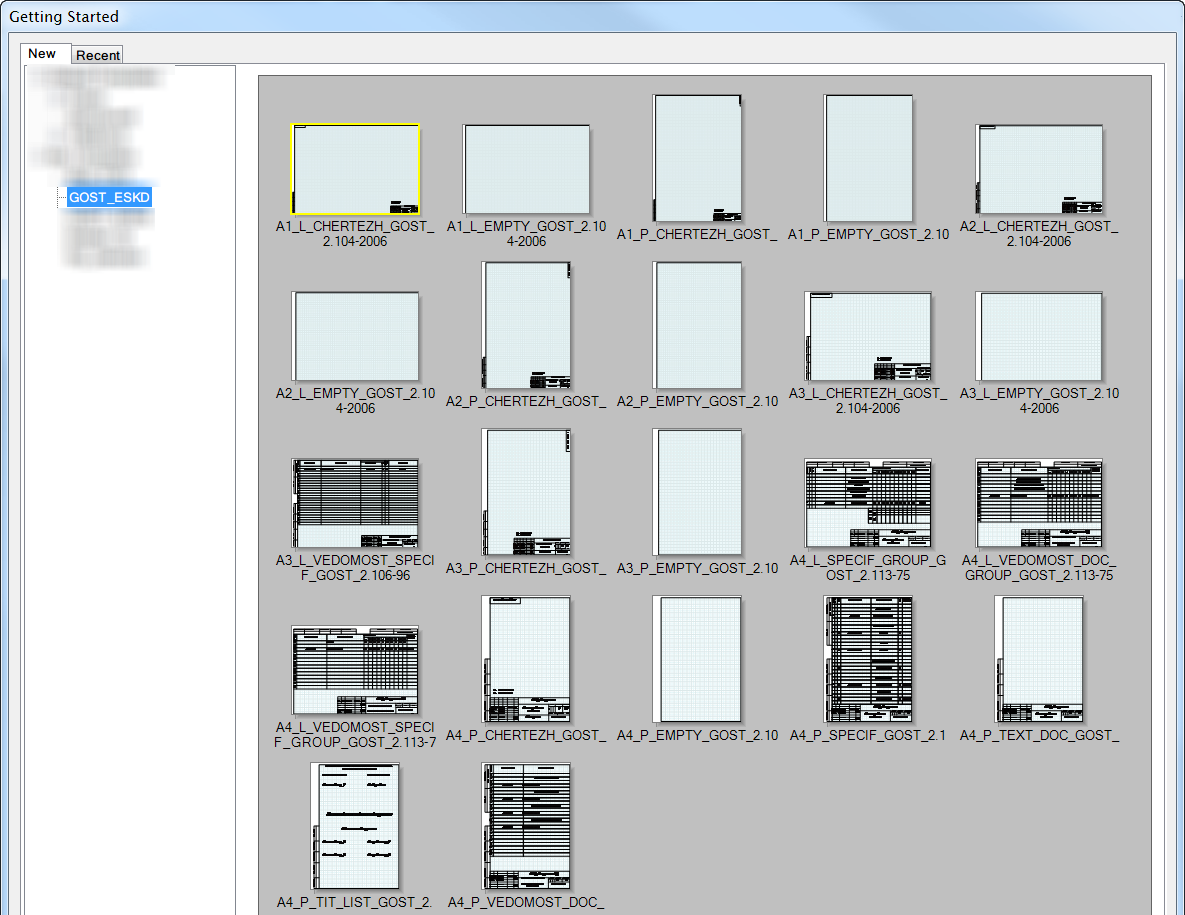
\includegraphics[width=\textwidth]{ESKD_NEW_FILE}
    \caption{Выбор шаблона ЕСКД.\label{ESKD_NEW_FILE}}
\end{figure}

\begin{figure}[t]
	\centering
	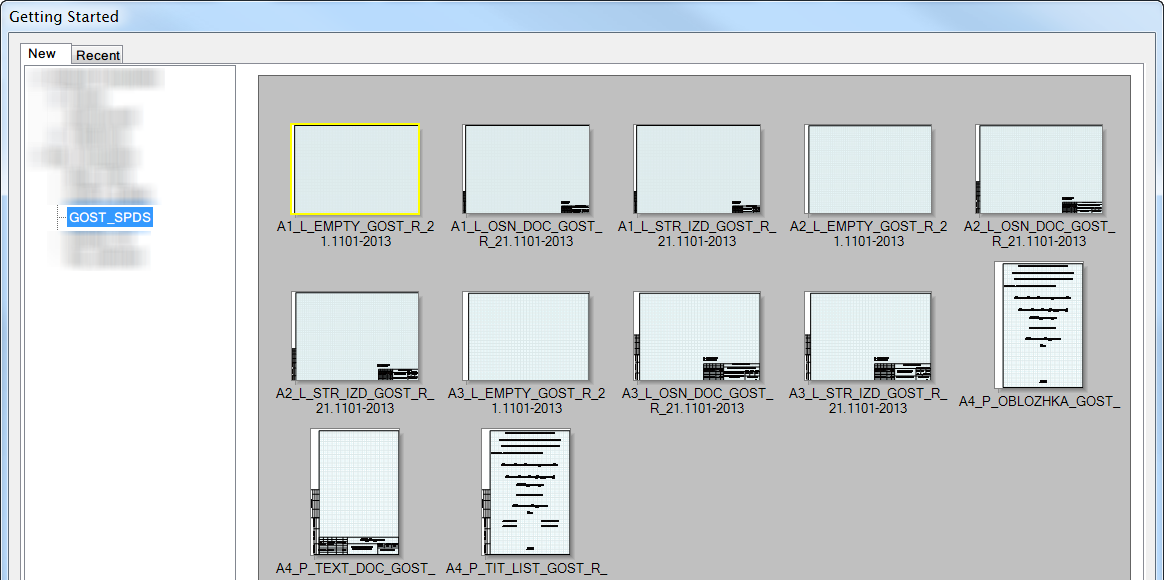
\includegraphics[width=\textwidth]{SPDS_NEW_FILE}
    \caption{Выбор шаблона СПДС.\label{SPDS_NEW_FILE}}
\end{figure}
\clearpage

Шаблон включает в себя один или два листа, в зависимости от типа документа. Создавать дополнительные листы необходимо на активном \textbf{последнем} листе документа через меню или аналогичными кнопками панели инструментов\\

\noindent
\menu[,]{Pages,Add} \\

\textbf{\emph{Примечание.}} Для шаблонов строительных чертежей основных комплектов (\textsf{OSN\_DOC}) необходимо копировать на новый лист содержимое слоя \textsf{OSNOVNAJA\_NADPIS\_VIEW}, который включает тег в графе 4 по форме 5 (\textsf{<Name\_View>} --- Наименование изображений помещенном на данном листе) и заполнять для каждого листа отдельно, изменив название самого тега, например \textsf{Name\_View\_Page}, где «\textsf{Page}» это номер страницы. Подробнее работа с тегами в данных шаблонах описана ниже.\\

Также в документах используются служебные слои. Названия слоев информируют об объектах, которые расположены на них. По умолчанию эти слои заблокированы.\\
Для заполнения \textbf{технических требований}, если таковые имеются, необходимо разблокировать слой «\textsf{TEH\_TREBOVANIJA}». Для перехода к следующему пункту жмем \keys{\enter}. Смена строки в текущем пункте происходит автоматически и определяется шириной блока текста.
Новые строки добавляются снизу. Первая  строка постоянно перемещается вверх.  Поэтому, для отображения всего, нужно сдвигать \textbf{только} верхнюю границу этого текстового блока. Слой рекомендуется заблокировать после ввода текста.\\

Для остальных полей применяется способ заполнения с помощью тегов («Auto-Text tags»)\footnote{\href{https://help.sketchup.com/en/layout/typing-importing-or-auto-inserting-text}{\uline{https://help.sketchup.com/en/layout/typing-importing-or-auto-inserting-text}}}. Их содержимое генерируется как автоматически (для номеров страниц, названий страниц) так и вводится вручную. Список тегов для каждого конкретного документа можно посмотреть в свойствах:\\

\noindent
\menu[,]{File,{Document Setup~\ldots},Auto-Text}\\

Правила заполнения основных надписей и других полей нужно смотреть в соответствующих стандартах. В приложениях~\ref{APP:ESKD} и~\ref{APP:SPDS} показаны теги, которые включены в файлы шаблонов, а так же размещение их в графах основной надписи.\\

Вместе с шаблонами поставляются готовые примеры в формате \emph{PDF}. Посмотреть их можно в каталоге по адресу:\\

\noindent
{\small \directory{Layout-GOST/Example\_PDF/Templates}}

\subsection{Scrapbooks}
В процессе оформления чертежа необходимо использовать блоки способом перетаскивания на лист документа («Drag and Drop»). При копировании свойств объектов из палитры \textsf{GOST\_SDPS} применяют инструмент \textsf{Style} («Пипетка»).
Все обозначение, кроме текстовых знаков, являются группой. Редактировать группу можно стандартными методами LayOut. Это перемещение объектов, масштабирование, изменения положения характерных точек линий («Двойной клик» по линии), стрелок, цвета, толщины и т.д.\\
Основные надписи, которые включены в Scrapbooks, имеют аналогичные теги, что и соответствующие формы шаблонов ЕСКД (Приложение~\ref{APP:ESKD}) и СПДС~(Приложение~\ref{APP:SPDS}).\\
:
Посмотреть примеры \textit{Scrapbooks} в формате \emph{PDF} можно в каталоге по адресу:\\

\noindent
\directory{Layout-GOST/Example\_PDF/Scrapbooks}\\

\begin{figure}[h]
	\centering
	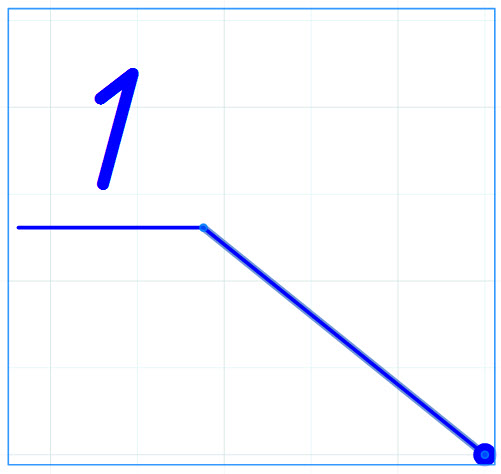
\includegraphics[width=0.35\textwidth]{ESKD_Point_1}
    \caption{Характерные точки линии.\label{ESKD_Point_1}}
\end{figure}

\begin{figure}[h]
	\centering
	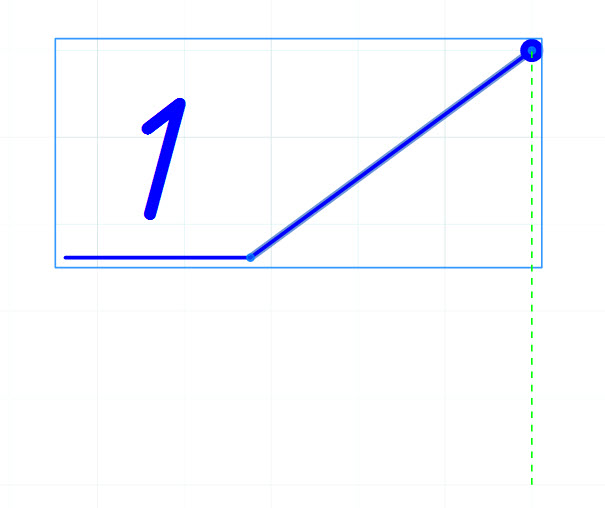
\includegraphics[width=0.35\textwidth]{ESKD_Point_2}
    \caption{Характерные точки линии после изменения положения.\label{ESKD_Point_2}}
\end{figure}


\appendix

\chapter{ЕСКД. Список тегов в шаблонах}
~\label{APP:ESKD}

\subsubsection{ГОСТ~2.104--2006}
\noindent
\begin{description}
	\item [Форма 1] --- Основная надпись для чертежей и схем (первый лист).
	\item [Форма 2] --- Основная надпись для текстовых конструкторских документов (первый лист).
	\item [Форма 2а] --- Основная надпись для чертежей (схем) и текстовых конструкторских документов (последующие листы).
\end{description}
Шаблон без основной надписи (\textsf{EMPTY}) включает с себя теги из шаблонов с основными надписями по формам 1 и 2а.

%Рисунки по Форме 1, 2а
\begin{figure}[h]
	\centering
	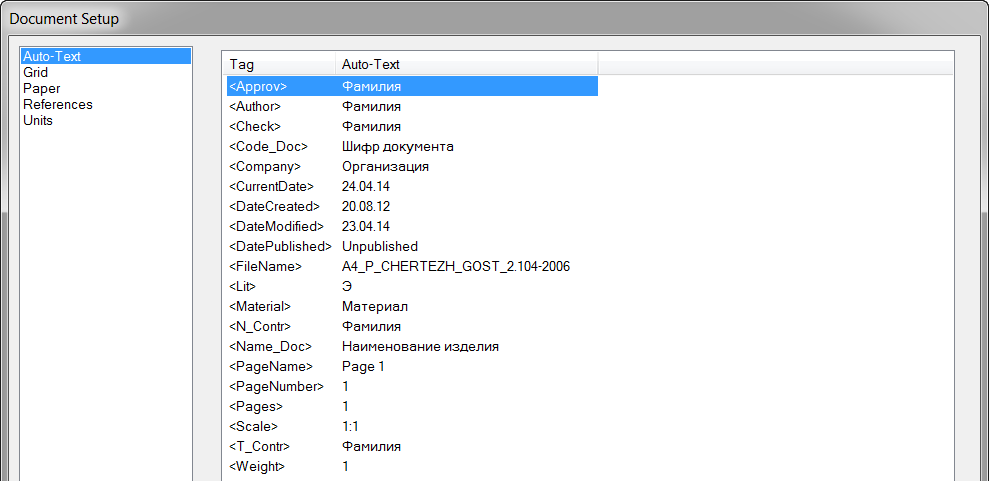
\includegraphics[width=\textwidth]{ESKD_CHERTEZH}
	\caption{Формы 1 и 2а. Список тегов основной надписи.\label{ESKD_CHERTEZH}}
\end{figure}

\begin{figure}[h]
	\centering
	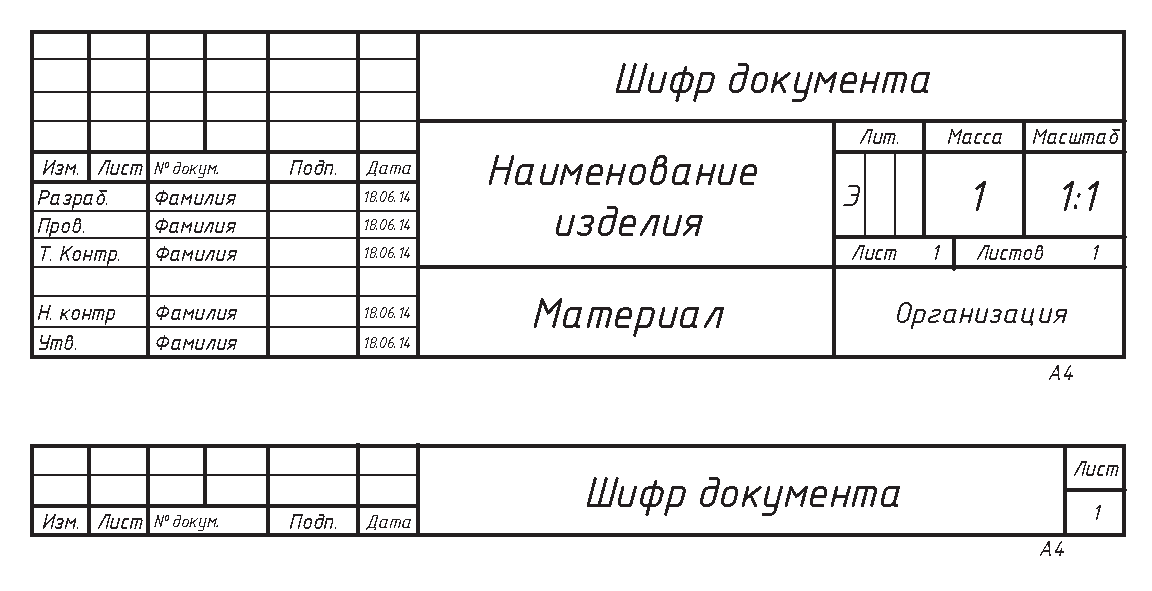
\includegraphics[width=\textwidth]{ESKD_CHERTEZH_without_tagname}
    \caption{Формы 1 и 2а. Заполнение граф основной надписи.\label{ESKD_CHERTEZH_without_tagname}}
\end{figure}

\begin{figure}[h]
	\centering
	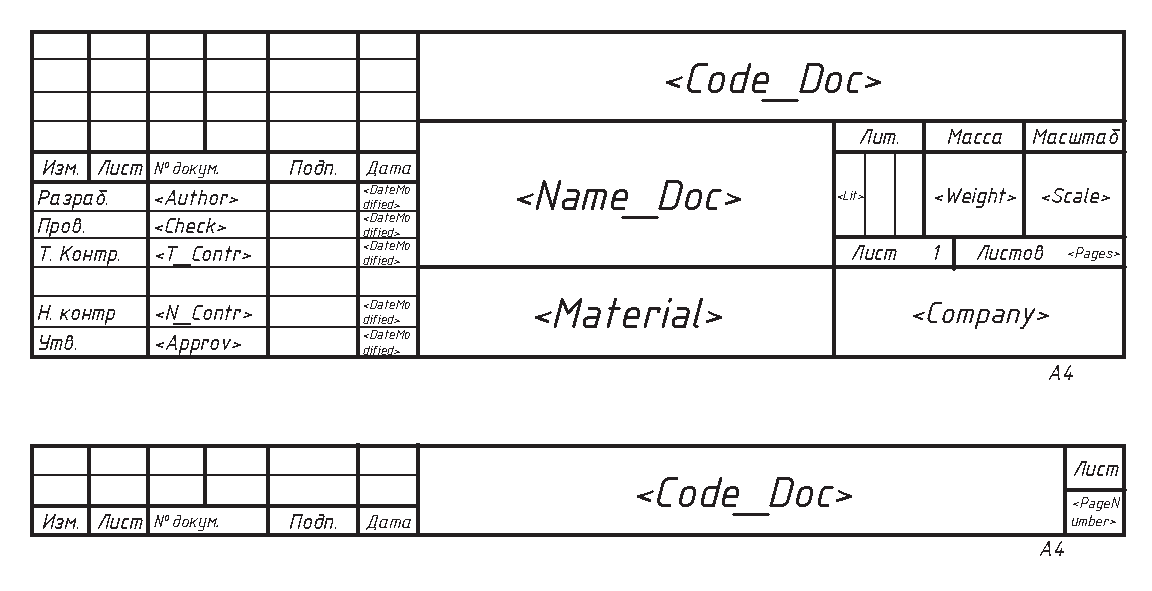
\includegraphics[width=\textwidth]{ESKD_CHERTEZH_with_tagname}
	\caption{Формы 1 и 2а. Соответствующие теги в графах основной надписи.\label{ESKD_CHERTEZH_with_tagname}}
\end{figure}

%Рисунки по Форме 2
\begin{figure}[h]
	\centering
	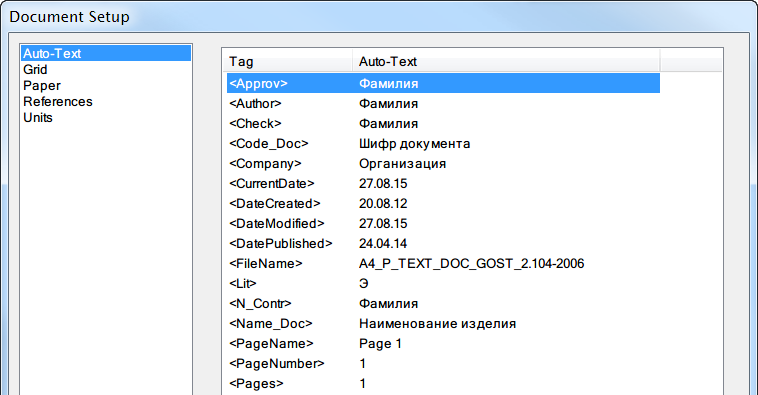
\includegraphics[width=\textwidth]{ESKD_TEXT_DOC}
    \caption{Формы 2 и 2а. Список тегов основной надписи.\label{ESKD_TEXT_DOC}}
\end{figure}

\begin{figure}[h]
	\centering
	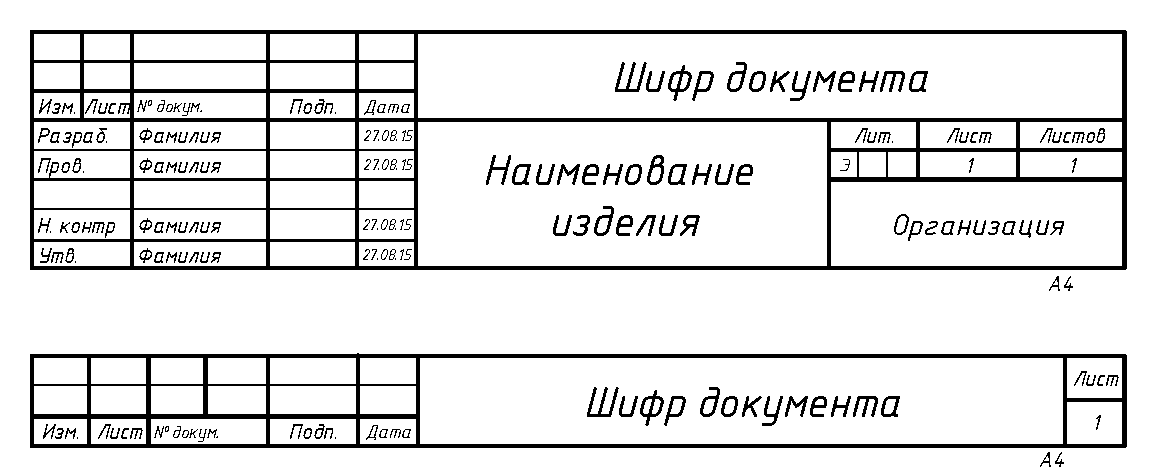
\includegraphics[width=\textwidth]{ESKD_TEXT_DOC_without_tagname}
	\caption{Формы 2 и 2а. Заполнение граф основной надписи.\label{ESKD_TEXT_DOC_without_tagname}}
\end{figure}

\begin{figure}[h]
	\centering
	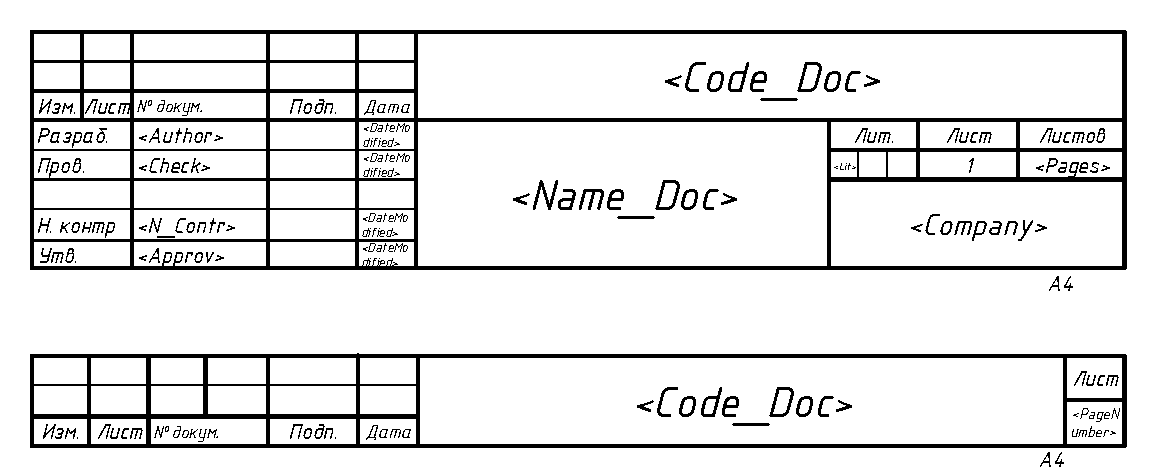
\includegraphics[width=\textwidth]{ESKD_TEXT_DOC_with_tagname}
    \caption{Формы 2 и 2а. Соответствующие теги в графах основной надписи.\label{ESKD_TEXT_DOC_with_tagname}}
\end{figure}

\begin{figure}[h]
	\centering
	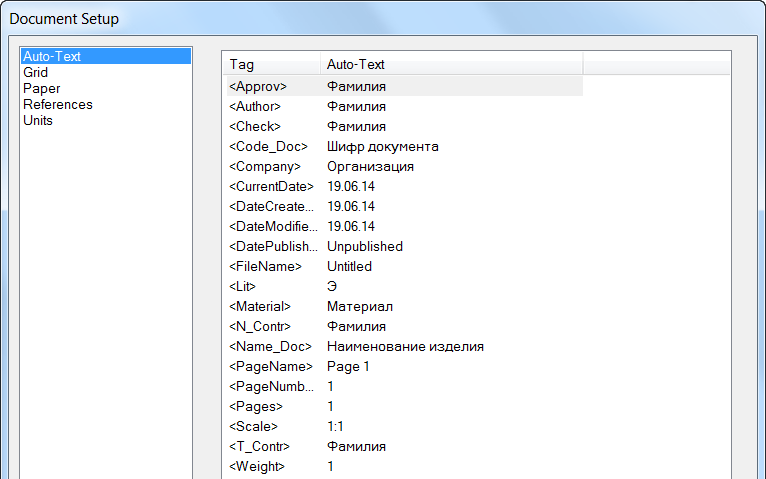
\includegraphics[width=0.8\textwidth]{ESKD_EMPTY}
	\caption{Список тегов шаблона без основной надписи\label{ESKD_EMPTY}}
\end{figure}
\clearpage

\subsubsection{ГОСТ~2.105--95}

\begin{figure}[h]
	\centering
	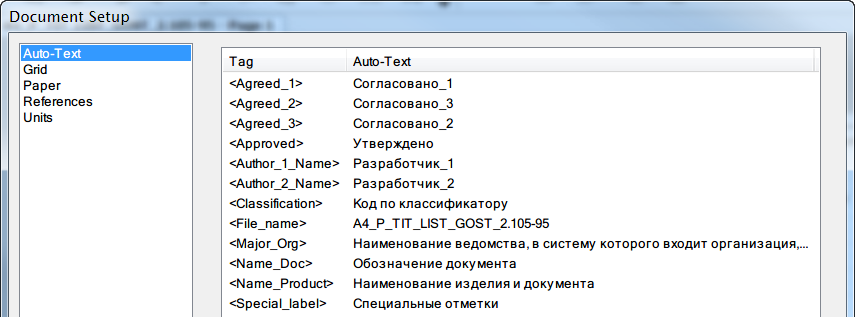
\includegraphics[width=\textwidth]{ESKD_TIT_LIST}
    \caption{Титульный лист. Список тегов.\label{ESKD_TIT_LIST}}
\end{figure}

\begin{figure}[h]
	\centering
	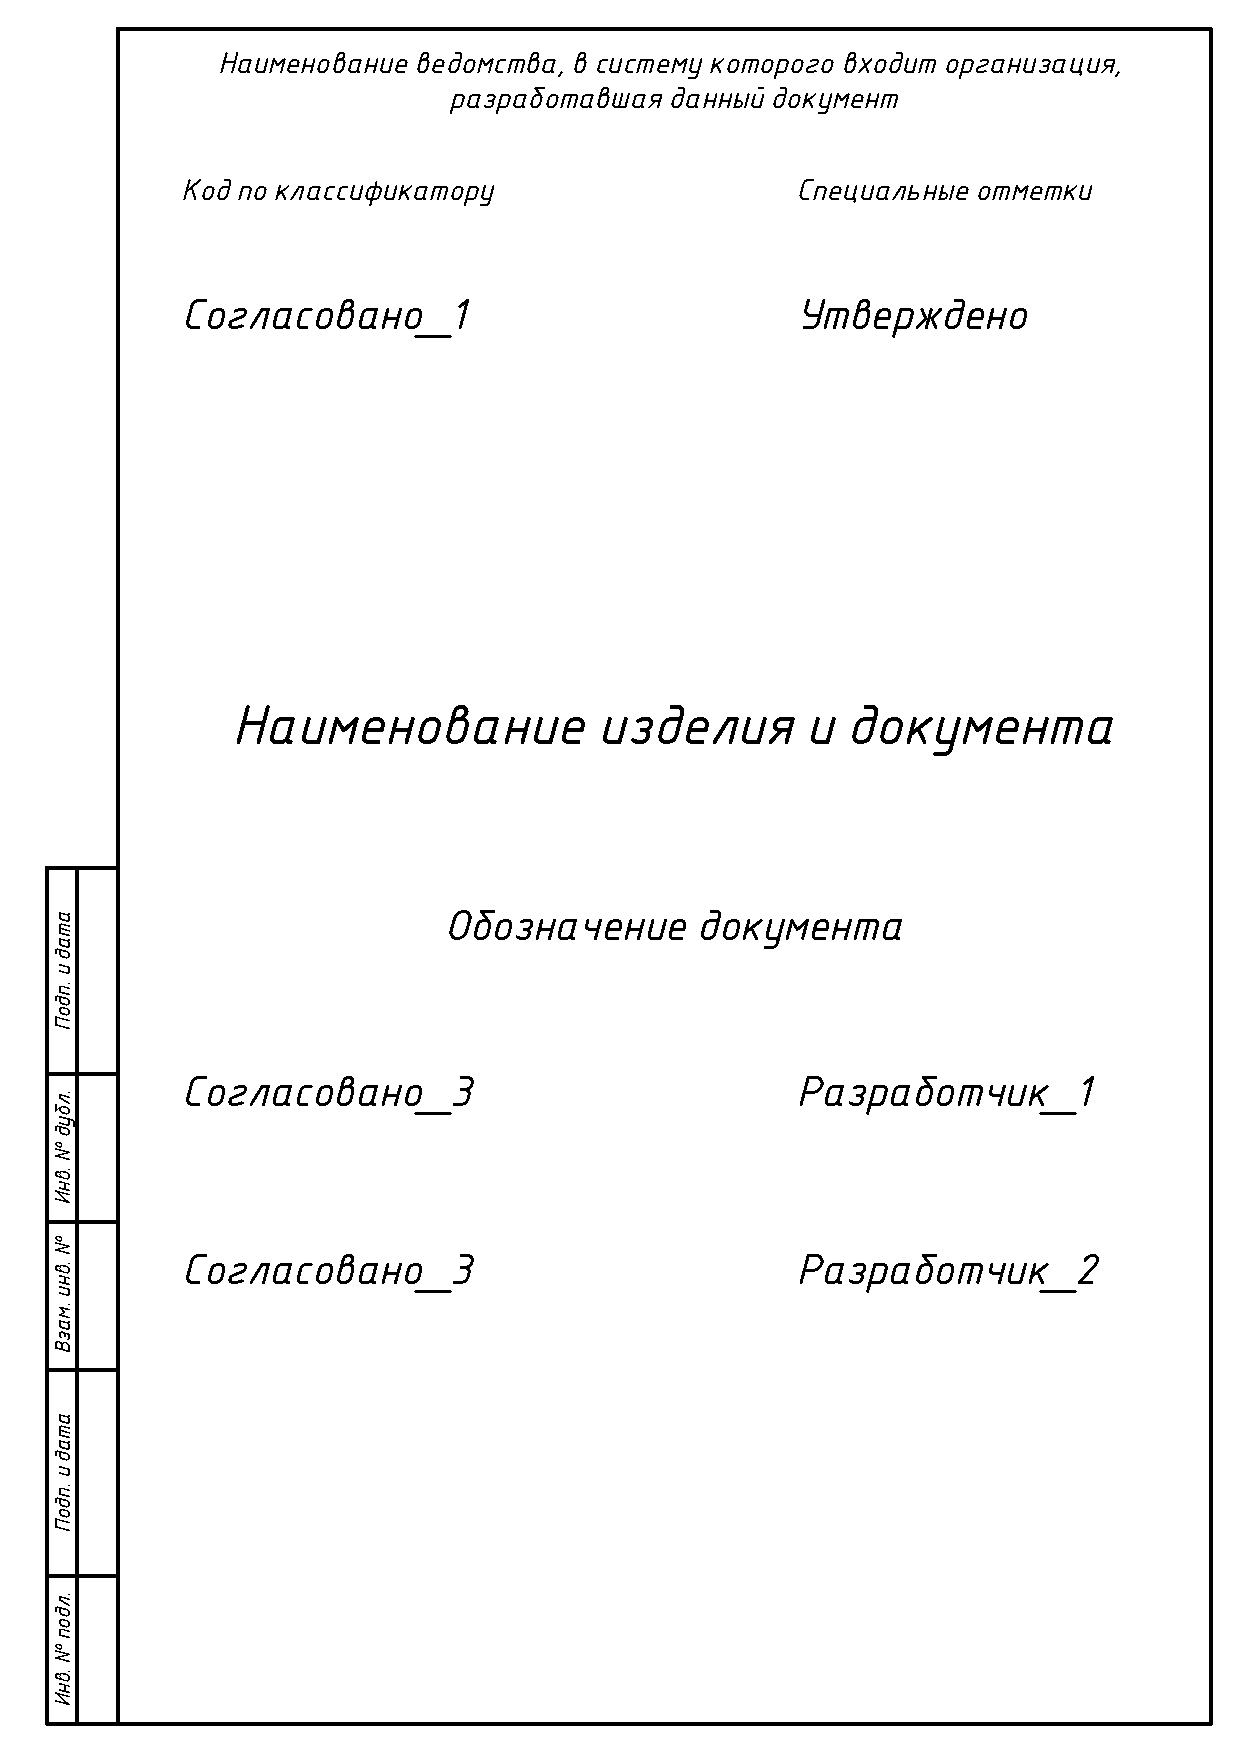
\includegraphics[width=\textwidth]{ESKD_TIT_LIST_without_tagname}
    \caption{Титульный лист. Заполнение граф.\label{ESKD_TIT_LIST_without_tagname}}
\end{figure}

\begin{figure}[h]
	\centering
	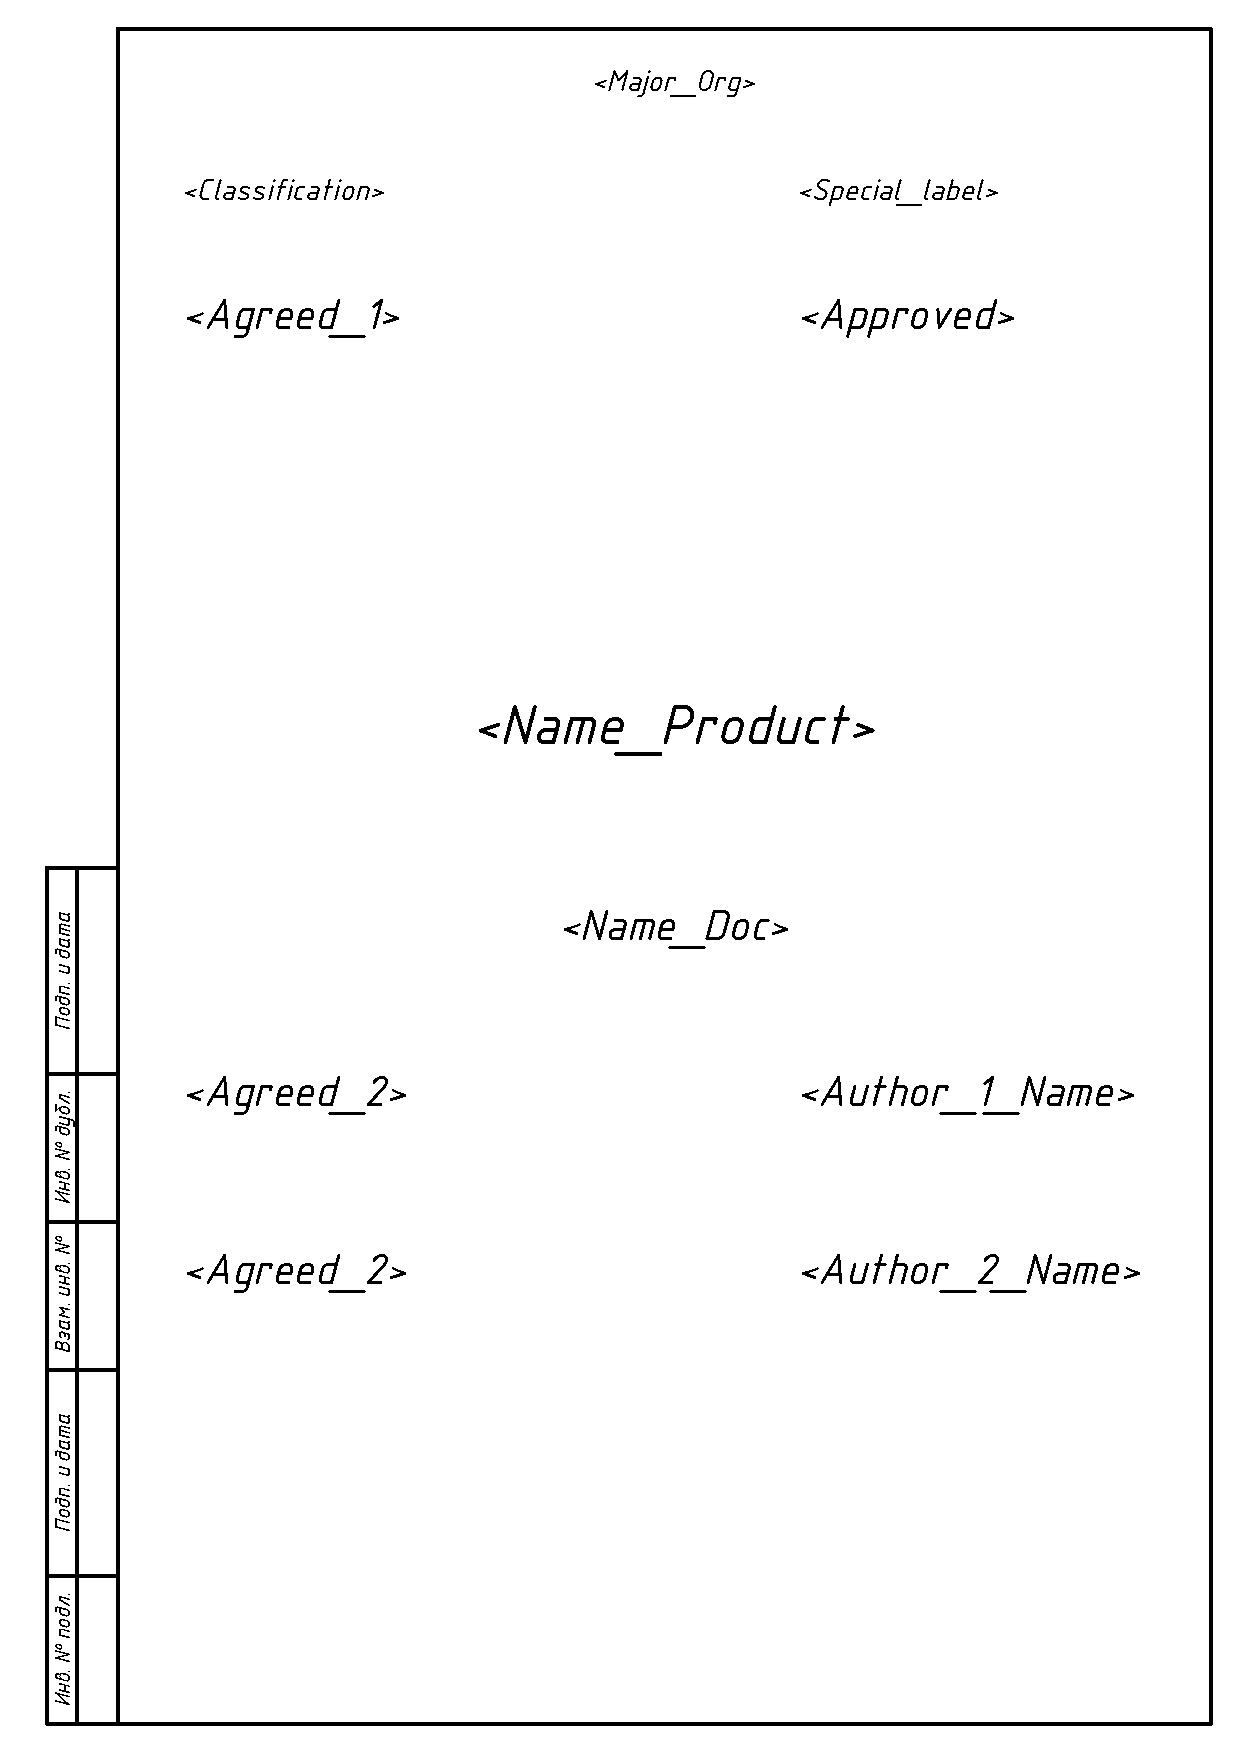
\includegraphics[width=\textwidth]{ESKD_TIT_LIST_with_tagname}
    \caption{Титульный лист. Соответствующие теги в графах.\label{ESKD_TIT_LIST_with_tagname}}
\end{figure}

\chapter{СПДС. Список тегов в шаблонах}
~\label{APP:SPDS}

\subsubsection{ГОСТ~21.1101--2013}
\noindent
\begin{description}
	\item [Форма 3] --- Для листов основных комплектов рабочих чертежей, графических документов проектной документации и графических документов по инженерным изысканиям.
	\item [Форма 4] --- Для чертежей строительных изделий (первый лист).
	\item [Форма 5] --- Для эскизных чертежей общих видов нетиповых изделий, всех видов текстовых документов (первый или заглавный лист).
	\item [Форма 6] --- Для чертежей строительных изделий, эскизных чертежей общих видов нетиповых изделий и всех видов текстовых документов (последующие листы).
	\item [Форма 12] --- Обложка.
	\item [Форма 13] --- Титульный лист.

\end{description}

Шаблон без основной надписи (\textsf{EMPTY}) включает с себя теги из шаблонов с основными надписями по формам 3, 4, 5 и 6.

%Рисунки по Форме 3
\begin{figure}[h]
	\centering
	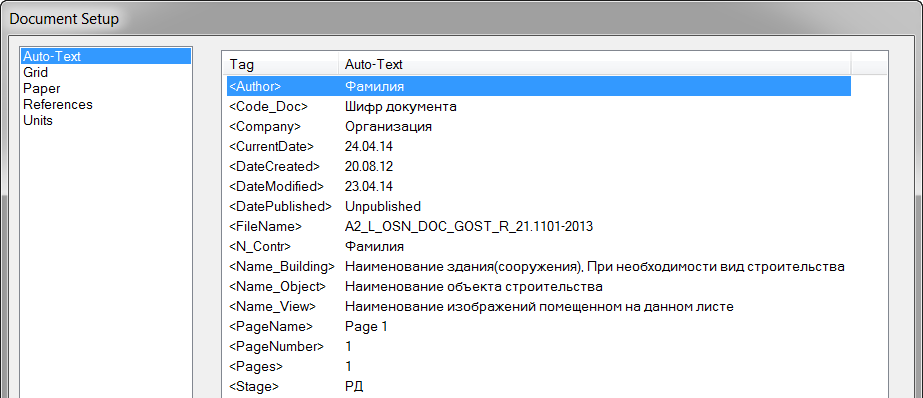
\includegraphics[width=0.8\textwidth]{SPDS_OSN_DOC}
    \caption{Форма 3. Список тегов основной надписи.\label{SPDS_OSN_DOC}}
\end{figure}

\begin{figure}[h]
	\centering
	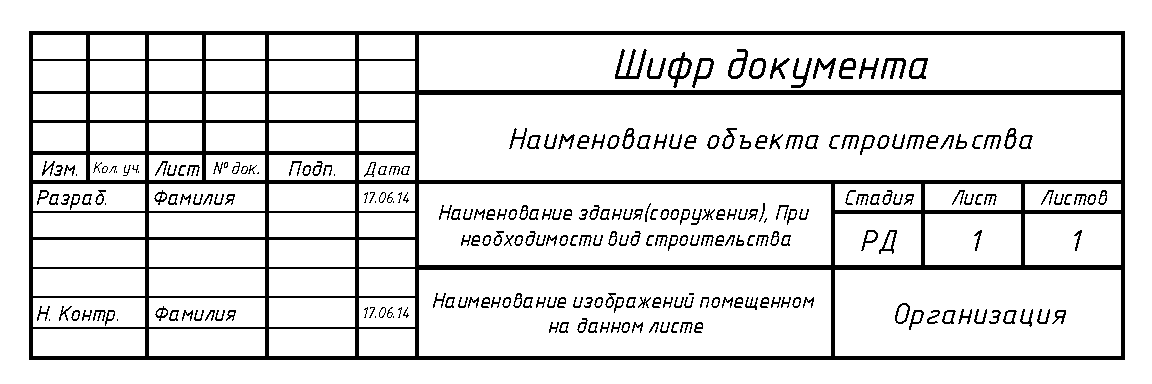
\includegraphics[width=\textwidth]{SPDS_OSN_DOC_without_tagname}
    \caption{Форма 3. Заполнение граф основной надписи.\label{SPDS_OSN_DOC_without_tagname}}
\end{figure}

\begin{figure}[h]
	\centering
	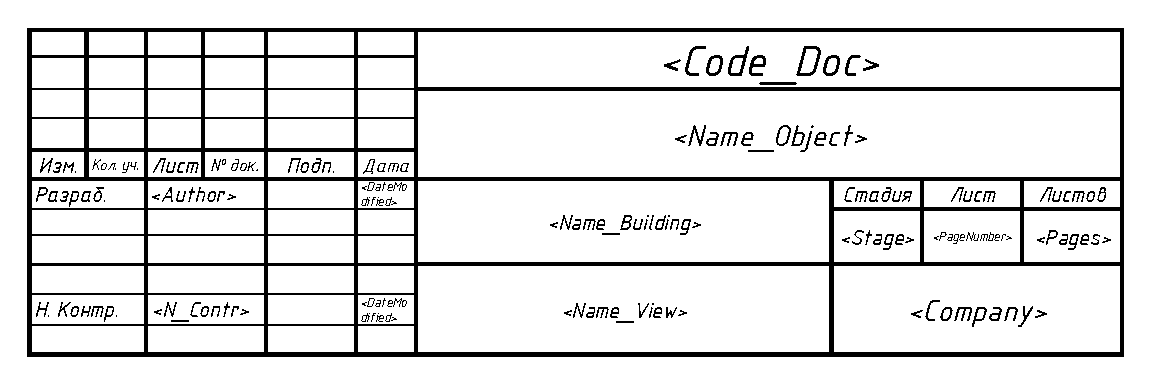
\includegraphics[width=\textwidth]{SPDS_OSN_DOC_with_tagname}
    \caption{Форма 3. Соответствующие теги в графах основной надписи.\label{SPDS_OSN_DOC_with_tagname}}
\end{figure}

%Рисунки по Формах 4 и 6
\begin{figure}[h]
	\centering
	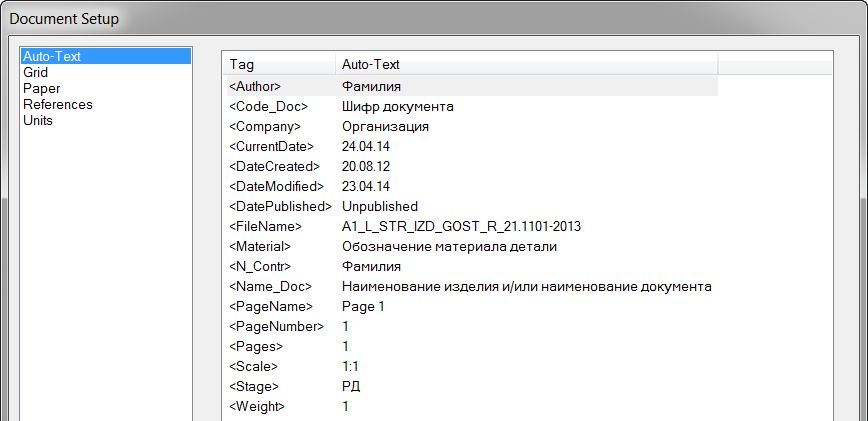
\includegraphics[width=\textwidth]{SPDS_STR_IZD}
    \caption{Формы 4 и 6. Список тегов основной надписи.\label{SPDS_STR_IZD}}
\end{figure}

\begin{figure}[h]
	\centering
	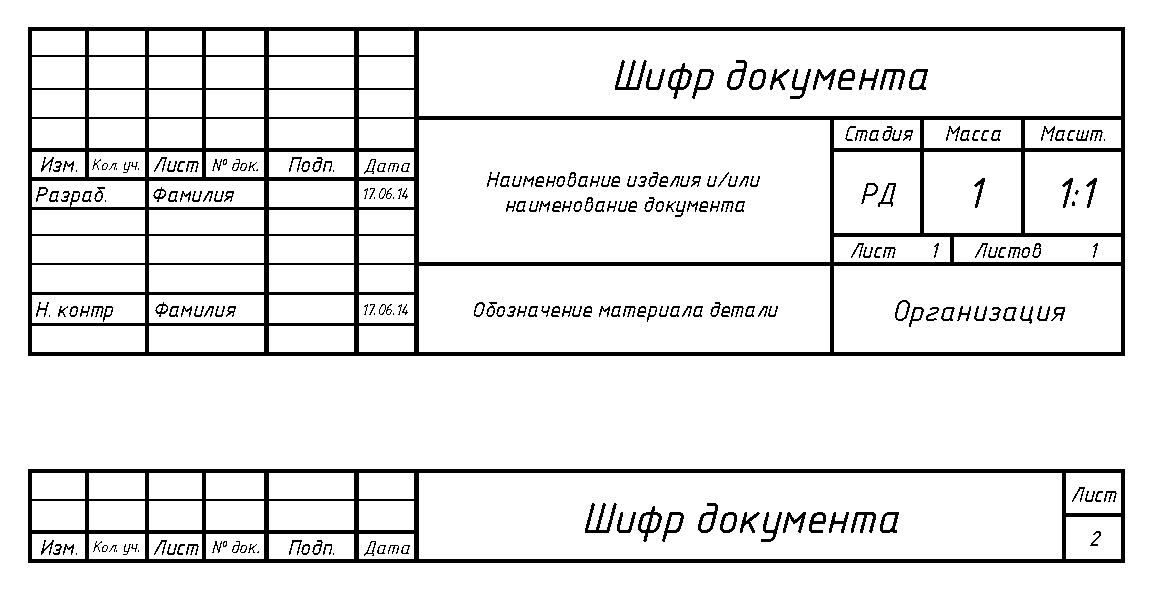
\includegraphics[width=\textwidth]{SPDS_STR_IZD_without_tagname}
    \caption{Формы 4 и 6. Заполнение граф основной надписи.\label{SPDS_STR_IZD_without_tagname}}
\end{figure}

\begin{figure}[h]
	\centering
	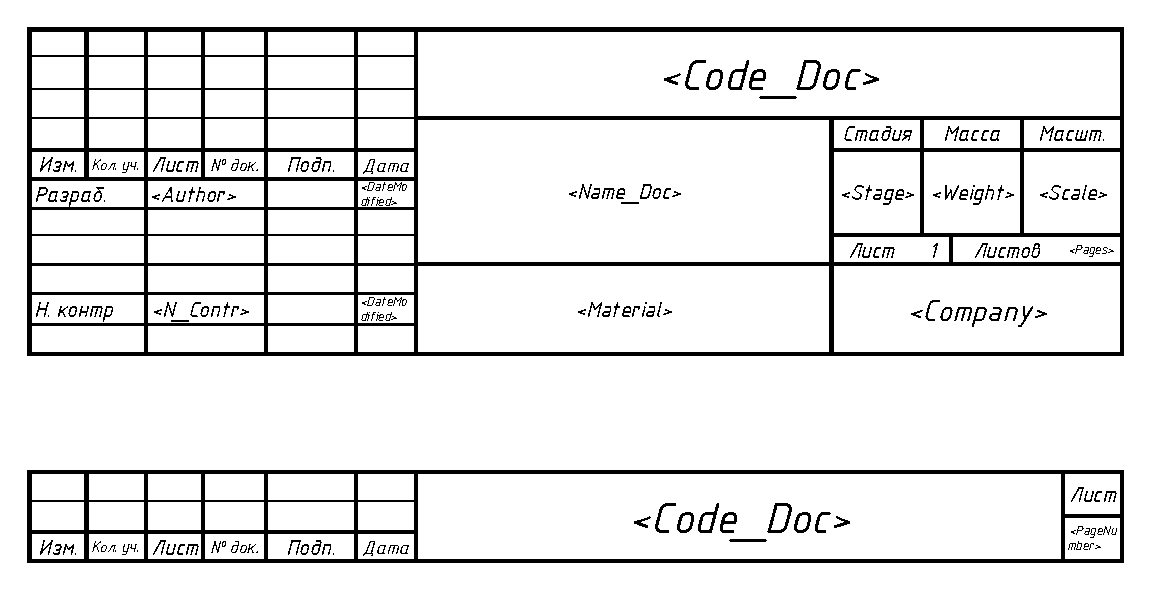
\includegraphics[width=\textwidth]{SPDS_STR_IZD_with_tagname}
	\caption{Формы 4 и 6. Соответствующие теги в графах основной надписи.\label{SPDS_STR_IZD_with_tagname}}
\end{figure}

%%Рисунки по Форме 5
\begin{figure}[h]
	\centering
	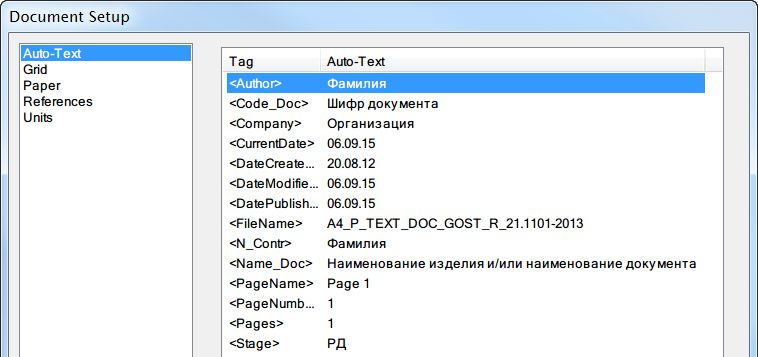
\includegraphics[width=\textwidth]{SPDS_TEXT_DOC}
	\caption{Форма 5. Список тегов основной надписи.\label{SPDS_TEXT_DOC}}
\end{figure}

\begin{figure}[h]
	\centering
	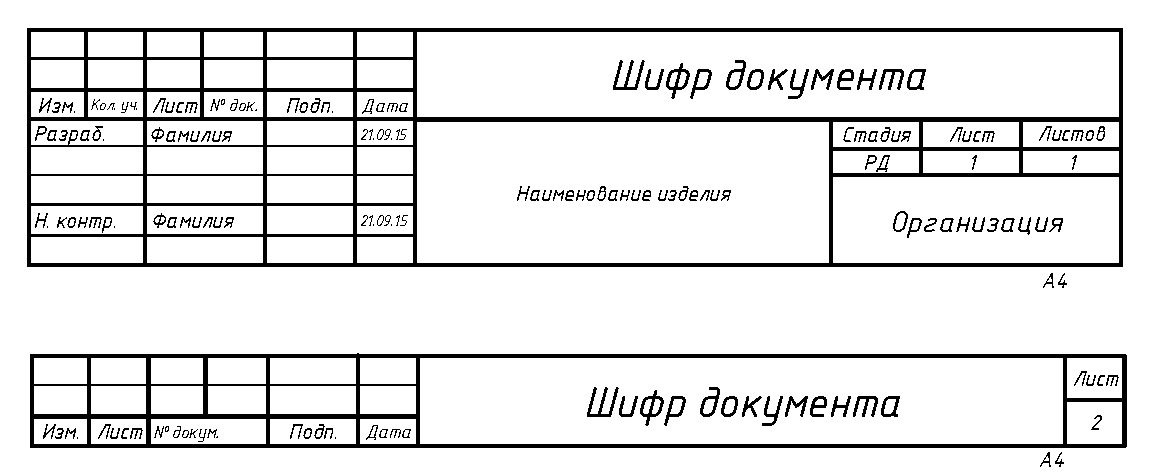
\includegraphics[width=\textwidth]{SPDS_TEXT_DOC_without_tagname}
	\caption{Формы 5. Заполнение граф основной надписи.\label{SPDS_TEXT_DOC_without_tagname}}
\end{figure}

\begin{figure}[h]
	\centering
	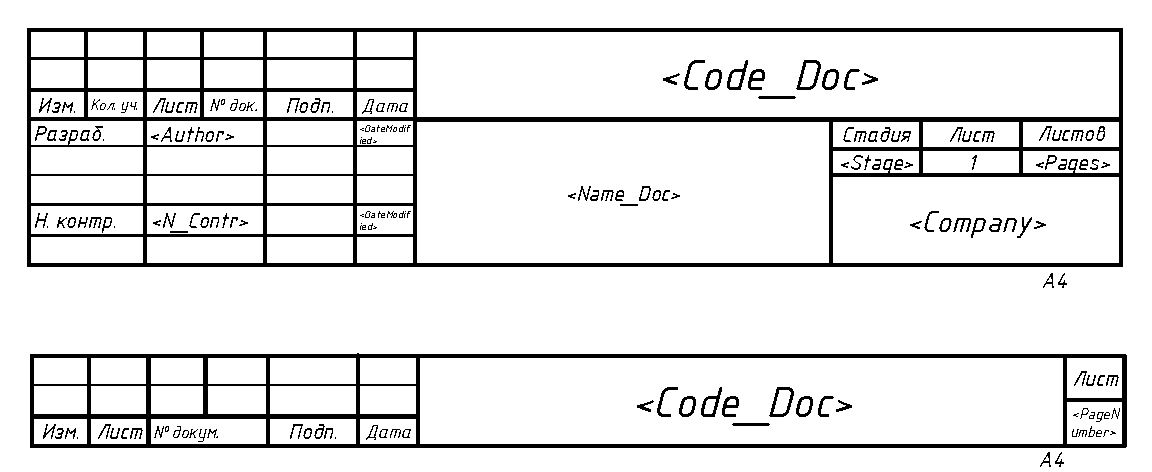
\includegraphics[width=\textwidth]{SPDS_TEXT_DOC_with_tagname}
    \caption{Формы 5. Соответствующие теги в графах основной надписи.\label{SPDS_TEXT_DOC_with_tagname}}
\end{figure}

%Рисунки по Форме 12
\begin{figure}[h]
	\centering
	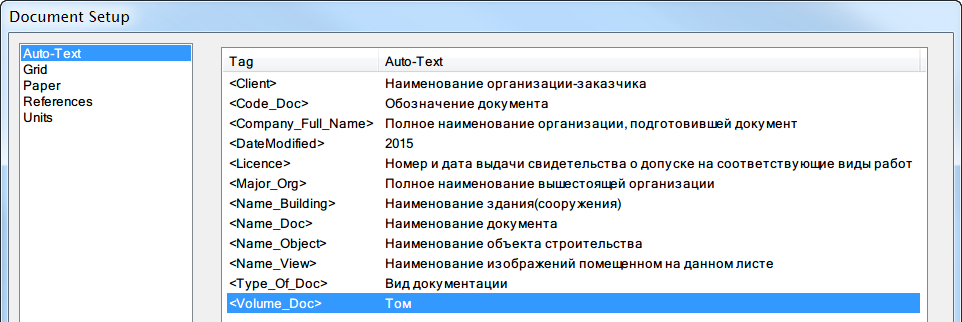
\includegraphics[width=0.8\textwidth]{SPDS_OBLOZHKA}
	\caption{Форма 12. Список тегов обложки.\label{SPDS_OBLOZHKA}}
\end{figure}

\begin{figure}[h]
	\centering
	
\includegraphics[width=0.9\textwidth]{SPDS_OBLOZHKA_without_tagname}
    \caption{Форма 12. Заполнение граф обложки.\label{SPDS_OBLOZHKA_without_tagname}}
\end{figure}

\begin{figure}[h]
	\centering
	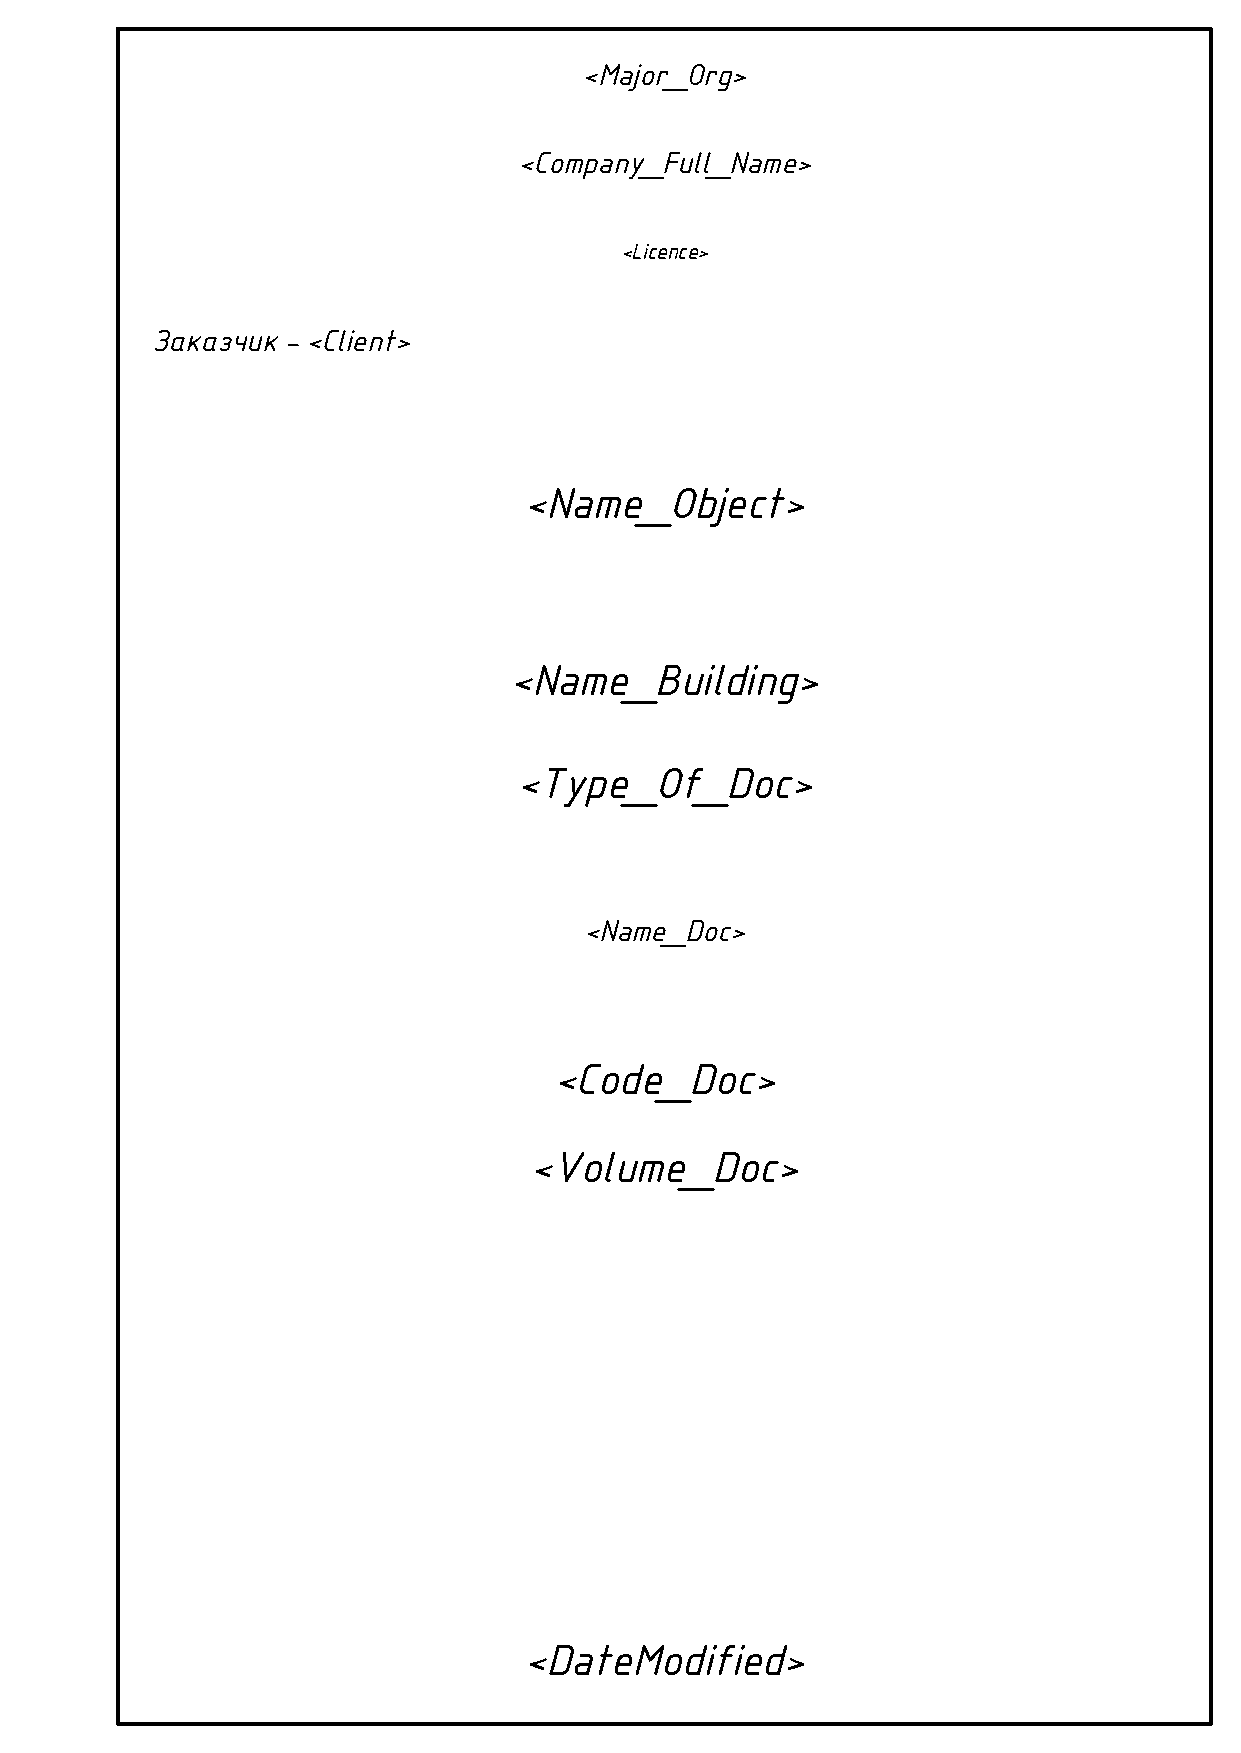
\includegraphics[width=0.9\textwidth]{SPDS_OBLOZHKA_with_tagname}
	\caption{Форма 12. Соответствующие теги в графах обложки.\label{SPDS_OBLOZHKA_with_tagname}}
\end{figure}

%Рисунки по Форме 13
\begin{figure}[h]
	\centering
	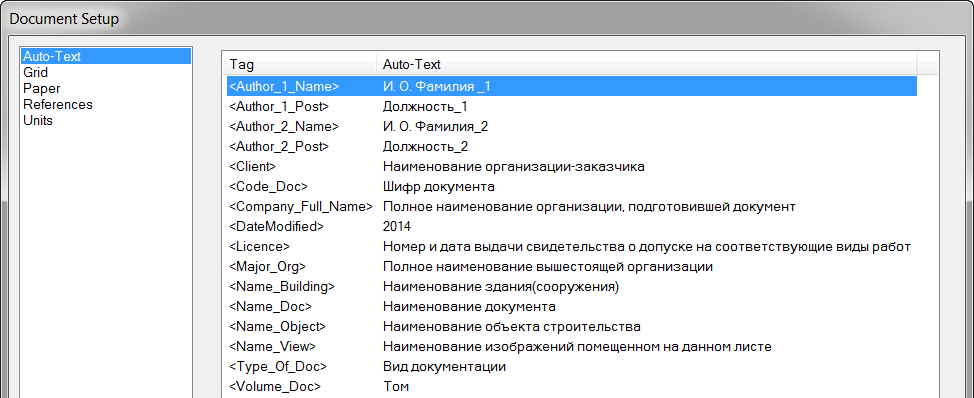
\includegraphics[width=0.8\textwidth]{SPDS_TIT_LIST}
    \caption{Форма 13. Список тегов титульного листа.\label{SPDS_TIT_LIST}}
\end{figure}

\begin{figure}[h]
	\centering
	
\includegraphics[width=0.9\textwidth]{SPDS_TIT_LIST_without_tagname}
    \caption{Форма 13. Заполнение граф титульного листа.\label{SPDS_TIT_LIST_without_tagname}}
\end{figure}

\begin{figure}[h]
	\centering
	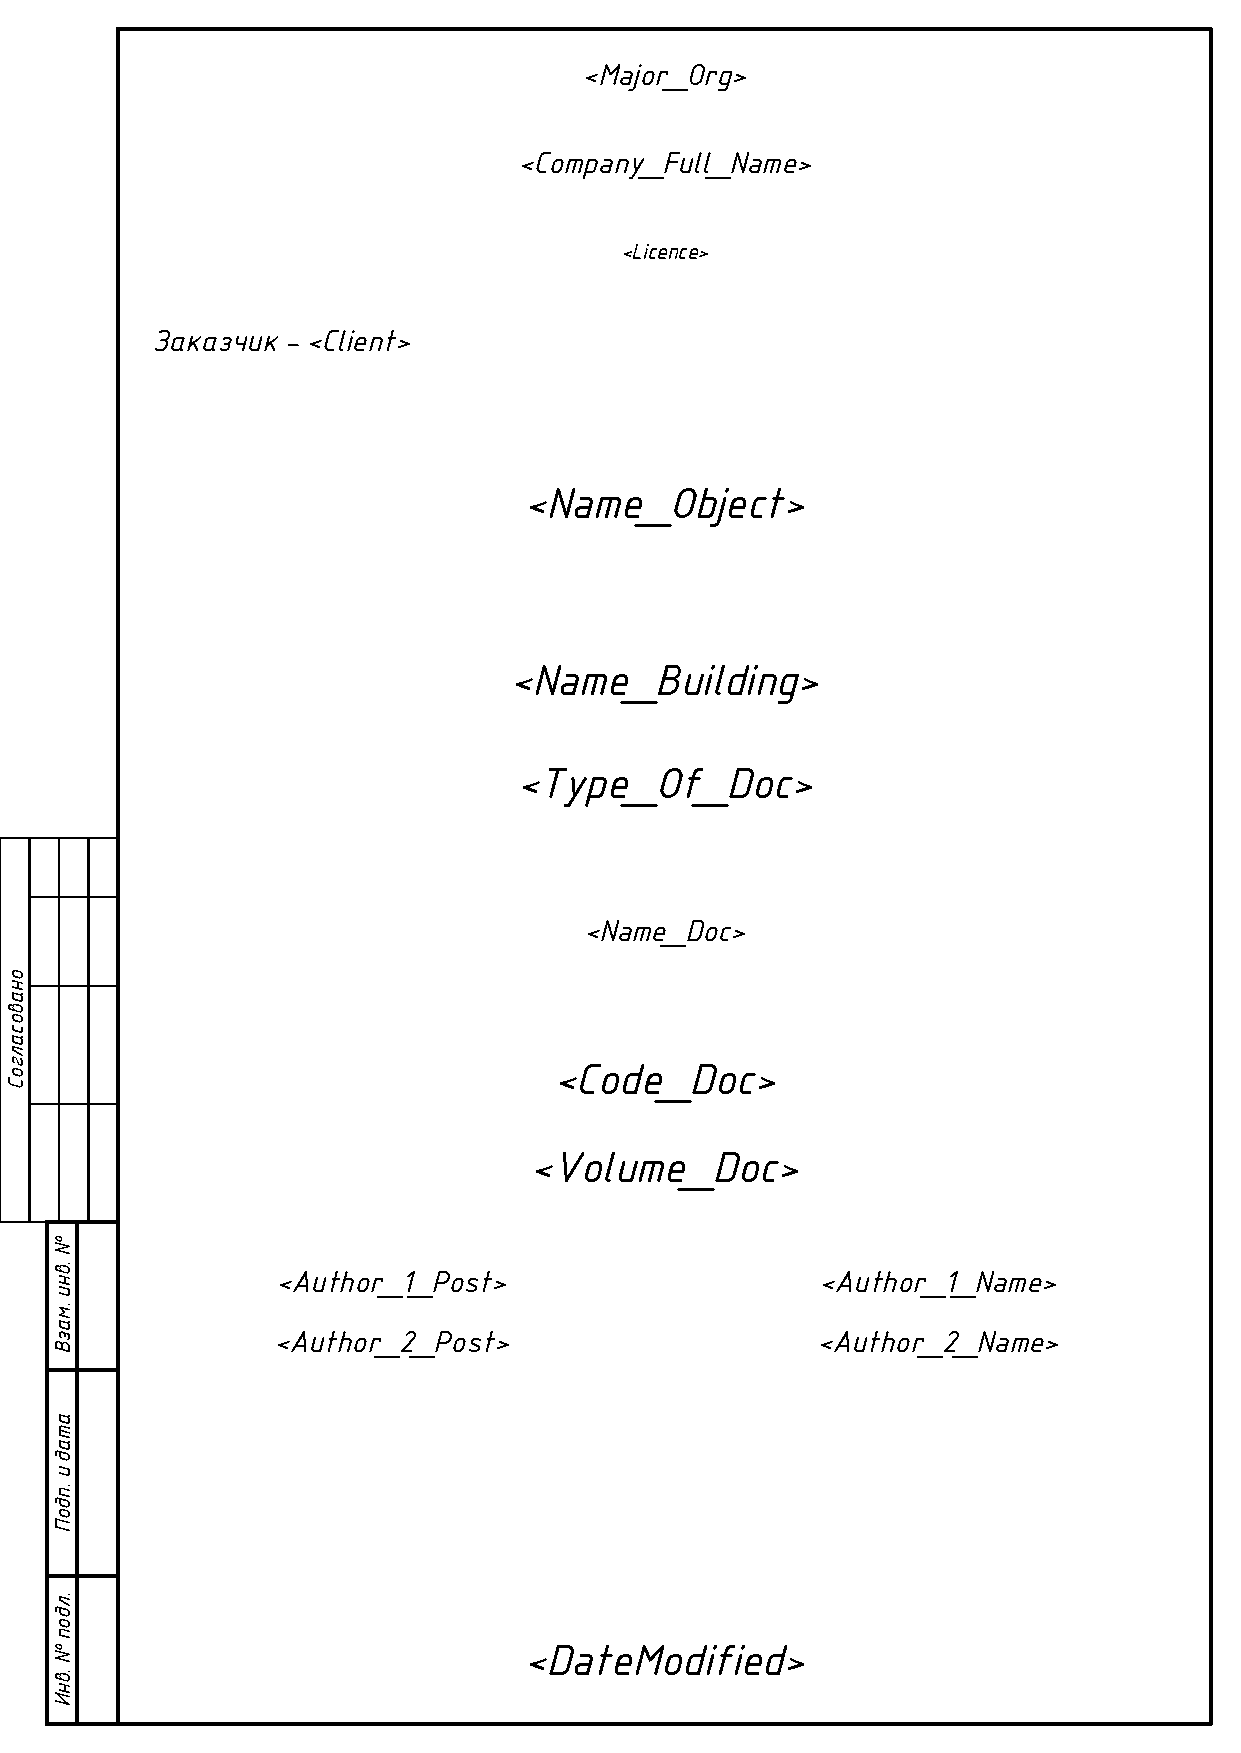
\includegraphics[width=0.9\textwidth]{SPDS_TIT_LIST_with_tagname}
    \caption{Форма 13. Соответствующие теги в графах титульного листа.\label{SPDS_TIT_LIST_with_tagname}}
\end{figure}

\begin{figure}[h]
	\centering
	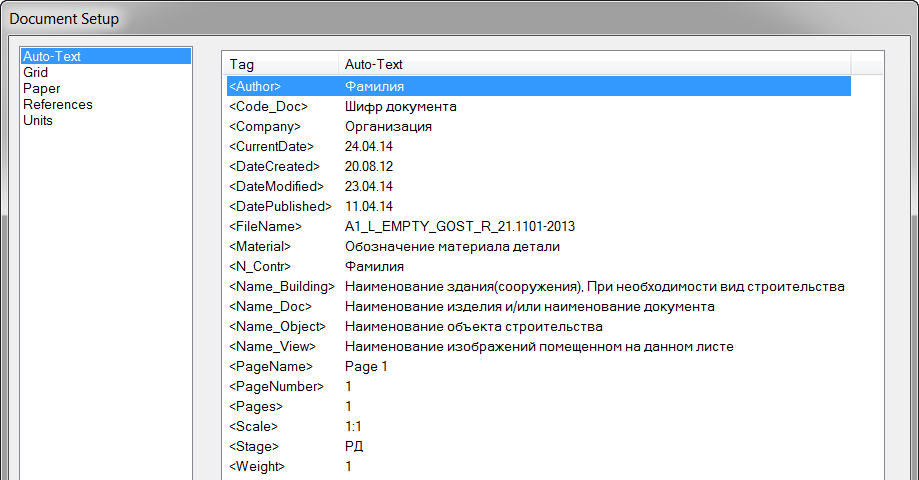
\includegraphics[width=0.8\textwidth]{SPDS_EMPTY}
    \caption{Список тегов шаблона без основной надписи.\label{SPDS_EMPTY}}
\end{figure}

\end{document}
